\documentclass[article,type=bsc,colorback,accentcolor=tud11d]{tudthesis}
\usepackage{ngerman}

\usepackage{varwidth}

\usepackage{graphicx}

% new page for each section
\usepackage{titlesec}
\newcommand{\sectionbreak}{\clearpage}

% flow charts etc.
\usepackage{tikz}
\usetikzlibrary{shapes,arrows,positioning,automata}

% increase line height
\renewcommand{\baselinestretch}{1.2} 


% german month for TUDthesis
\newcommand{\getmydate}{%
  \ifcase\month%
    \or Januar\or Februar\or M\"arz%
    \or April\or Mai\or Juni\or Juli%
    \or August\or September\or Oktober%
    \or November\or Dezember%
  \fi\ \number\year%
}

%--------------------------------------------------------------------------------

\begin{document}

% Meta Data for the title page
  \thesistitle{Optimierte Zusammenarbeit von HTTP/2 und Multipath-TCP-Schedulern}{Optimizing Cooperation of HTTP/2 and the Multipath TCP Scheduler}
  \author{Maxi Weller}
  \referee{Prof. Ralf Steinmetz}{Alexander Fr�mmgen}
  \department{Fachbereich Informatik}
  \group{Multimedia Communications Lab }
  \tuprints{57580}{5758}
  \makethesistitle
  \affidavit{M. Weller}


  \section*{Abstract}
abtract

\renewcommand{\contentsname}{Contents}
 \tableofcontents

  \section{Introduction}
intro

  \section{Related Work}
related work

  \subsection{Measuring Web Performance}
\cite{han2015mwebmptcp}


  \subsection{Optimizing HTTP}
(web performance? http2 performance?)
\cite{klotski2015}
(also, general article about HTTP/2 as optimization of http)
\cite{rfc7540}


  \subsection{Optimizing Multipath TCP Scheduling}
\cite{multipathtcp}


  \subsection{Cooperation of HTTP Server and TCP Stack}
(or more general, application layer and transport layer?)

\cite{Raisinghani_2004}
\cite{nowlan2012unorderedtcp}

\section{Multipath TCP}

\section{HTTP 2}


\section{Approaches for optimization}

Several optimization approaches are considered in this chapter.

\subsection{Switching the scheduler based on content type or priority}
Many modern web pages consist of dozens of resources. They can be classified by their technical priority for rendering the page. 

1. The \textit{Document} is the main HTML file which is loaded first. It is strictly necessary for the browser to render the page, and to load subsequent resources. 

2. Synchronous Javascript resources (\texttt{<script>} tags) are required by the browser to construct the Document Object Model (DOM) tree. They must be loaded as soon as the tag is parsed by the browser.

3. Style sheets are needed for the first layout cycle of the page, which means usually nothing is displayed to the user until they are fully loaded.

4. Images can be loaded after the base frame of the site is visible, especially if the image size is provided in the Document source. The same is true for video, audio and most AJAX requests.

...

One can also look at their subjective utility to the user.

In the case of text heavy pages, like news sites, the Document and some images are most useful to the user as that contains the content of the page. In these cases, the Javascript resources are often providing tracking and advertising, so very important for the webmaster but annoying for the user. Especially tracking scripts can be delivered with lower priority as they are invisible and not time critical.

For interactive pages, the Javascript might provide all the relevant contents.   

...  ... 

Modern browsers and speed-optimized web pages make sure that the resources with the highest technical priority are requested first. The HTTP/2 server can also facilitate this by pushing out high-priority resources with HTTP Push.

The resources required for the first layout cycle will be handled by a scheduler with emphasis on low latency, like a redundant scheduler on lossy connections. The redundant scheduler sends all segments out on all paths to minimize delays caused by packet loss.

After these high priority resources are sent out, a regular, more bandwidth conserving scheduler can be used.



\subsection{Aggressive transmission of last segments}
The transmitting application signals the state of its outgoing buffers to the scheduler. An interesting condition occurs when the HTTP server has no more data to send, and only a few segments are left in the scheduler's queue. This means only these few segments are missing so that a complete web page can be rendered for the user. The scheduler can try to push out the missing segments more aggressively: By temporarily ignoring the available congestion window for the left over bytes, or by retransmitting on all available subflows.



\section{Choosing a web server platform}

To get information about the contents of the HTTP/2 application data, the cooperation of the web server is required.



\section{Implementation}

The scheduler algorithms are implemented in a scripting language. The scripts are just-in-time compiled and interpreted by the Rule Based Scheduler.



\begin{figure}[b]
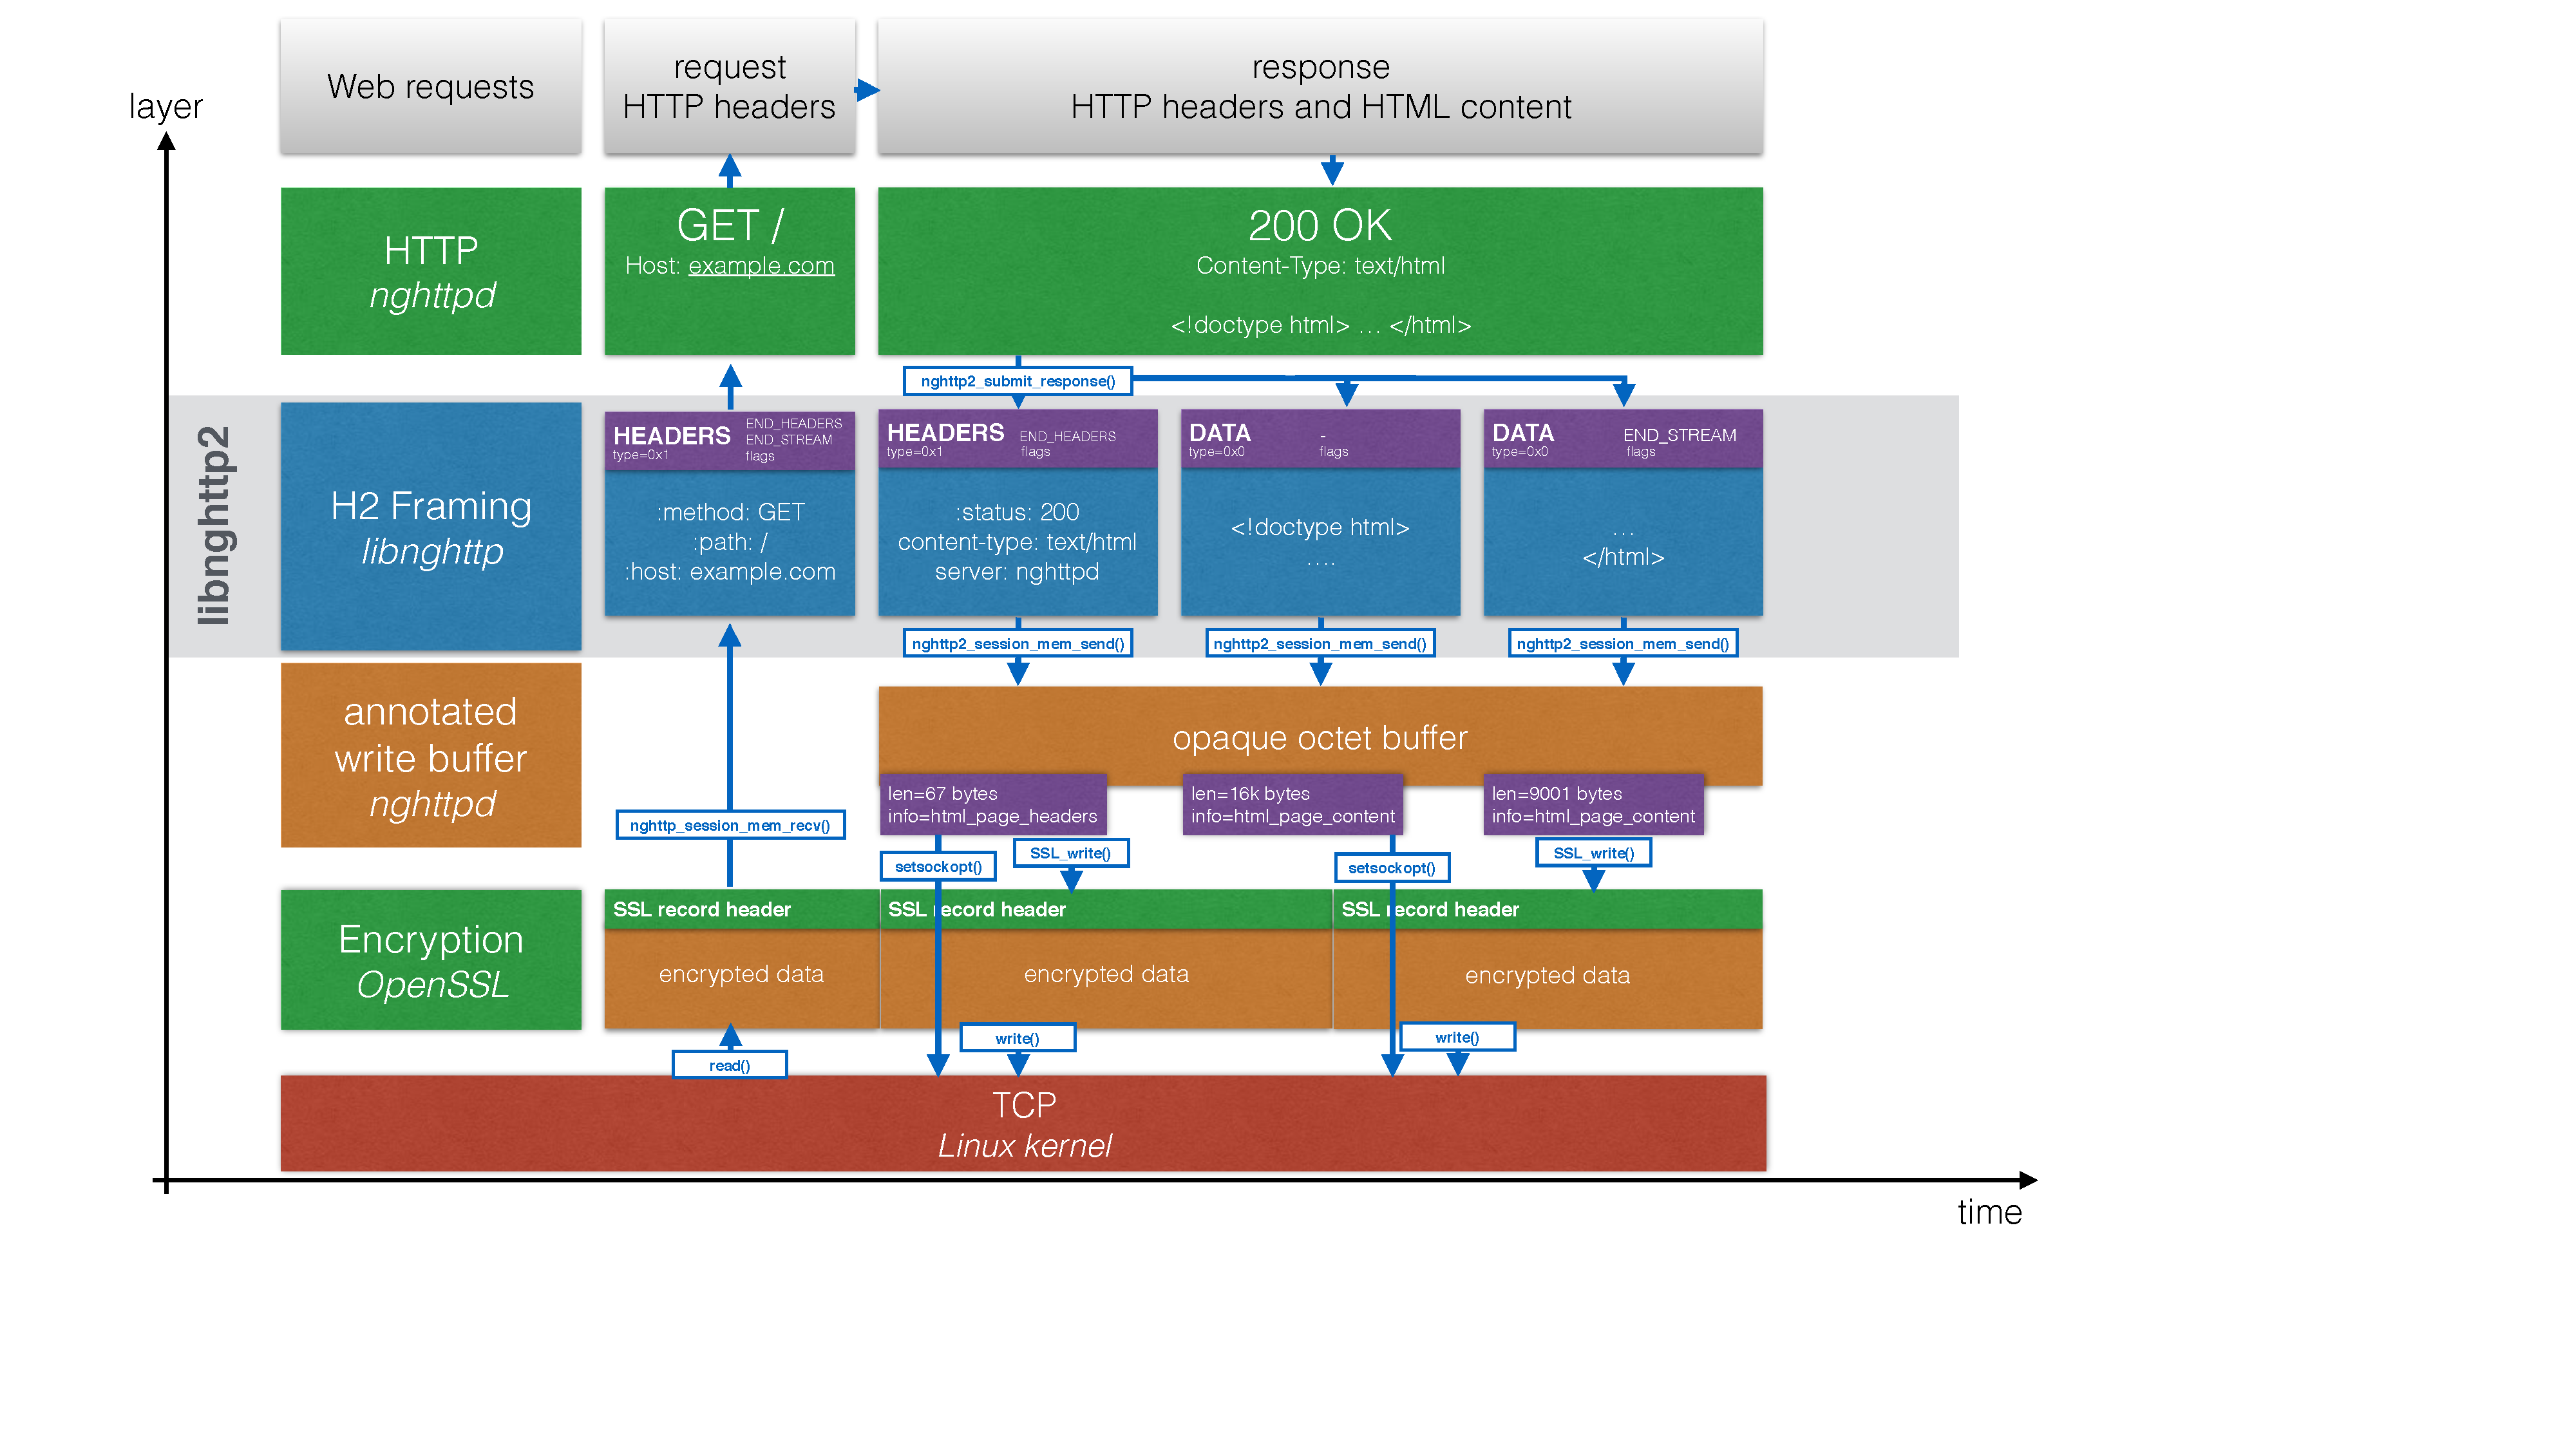
\includegraphics[width=1\textwidth]{http2-awb-layers.pdf}
  \caption{The annotated data's path through the application and network layer}
\end{figure}



\section{Evaluation}
One has to decide which web sites to measure, and how to measure them.


\subsection{Selection of sample web pages}


- Self built test pages (plain html, small html file with many scripts/css, big html, etc ...)


Measuring the page load times of real-world web pages:

- Alexa Top Sites (or similar ranking)

- Hand-selected sites with interesting features / problems / optimization potentials

- Sites which are often used on mobile


\subsection{Handling dynamic and third party requests}

Downloading web pages with browser / wget and delivering with nghttpd - Problem: how to handle dynamic or third-party requests?

\begin{itemize}
\item Cancel/reject all third party requests (in-browser / iptables)

Pro: Easy, reproducible

Con: not realistic (always a lot faster than real request)

Pro: might be faster by the same amount, so still comparable (?)

\item Let all third party requests through to the original sites

Pro: Easy, realistic

Con: dependent on network condition of test computer and load on original server (not reproducible)

\end{itemize}

Alternative: Use a caching HTTP/2 proxy (nghttpx, apache)

Pro: realistic (?), reproducible, (not that difficult either)

Con: ...



\section{HTTP/2}


\subsection{Page Load Speed Measurements}


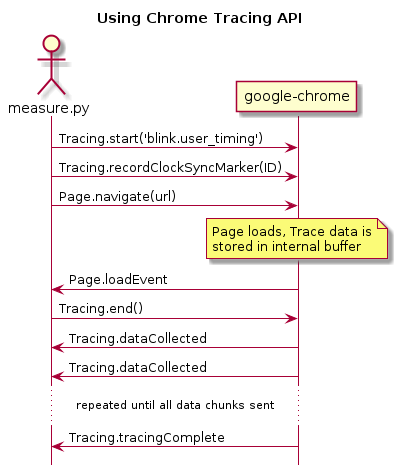
\includegraphics{chrome-tracing-api.png}


\subsection{Streams}
% Define block styles

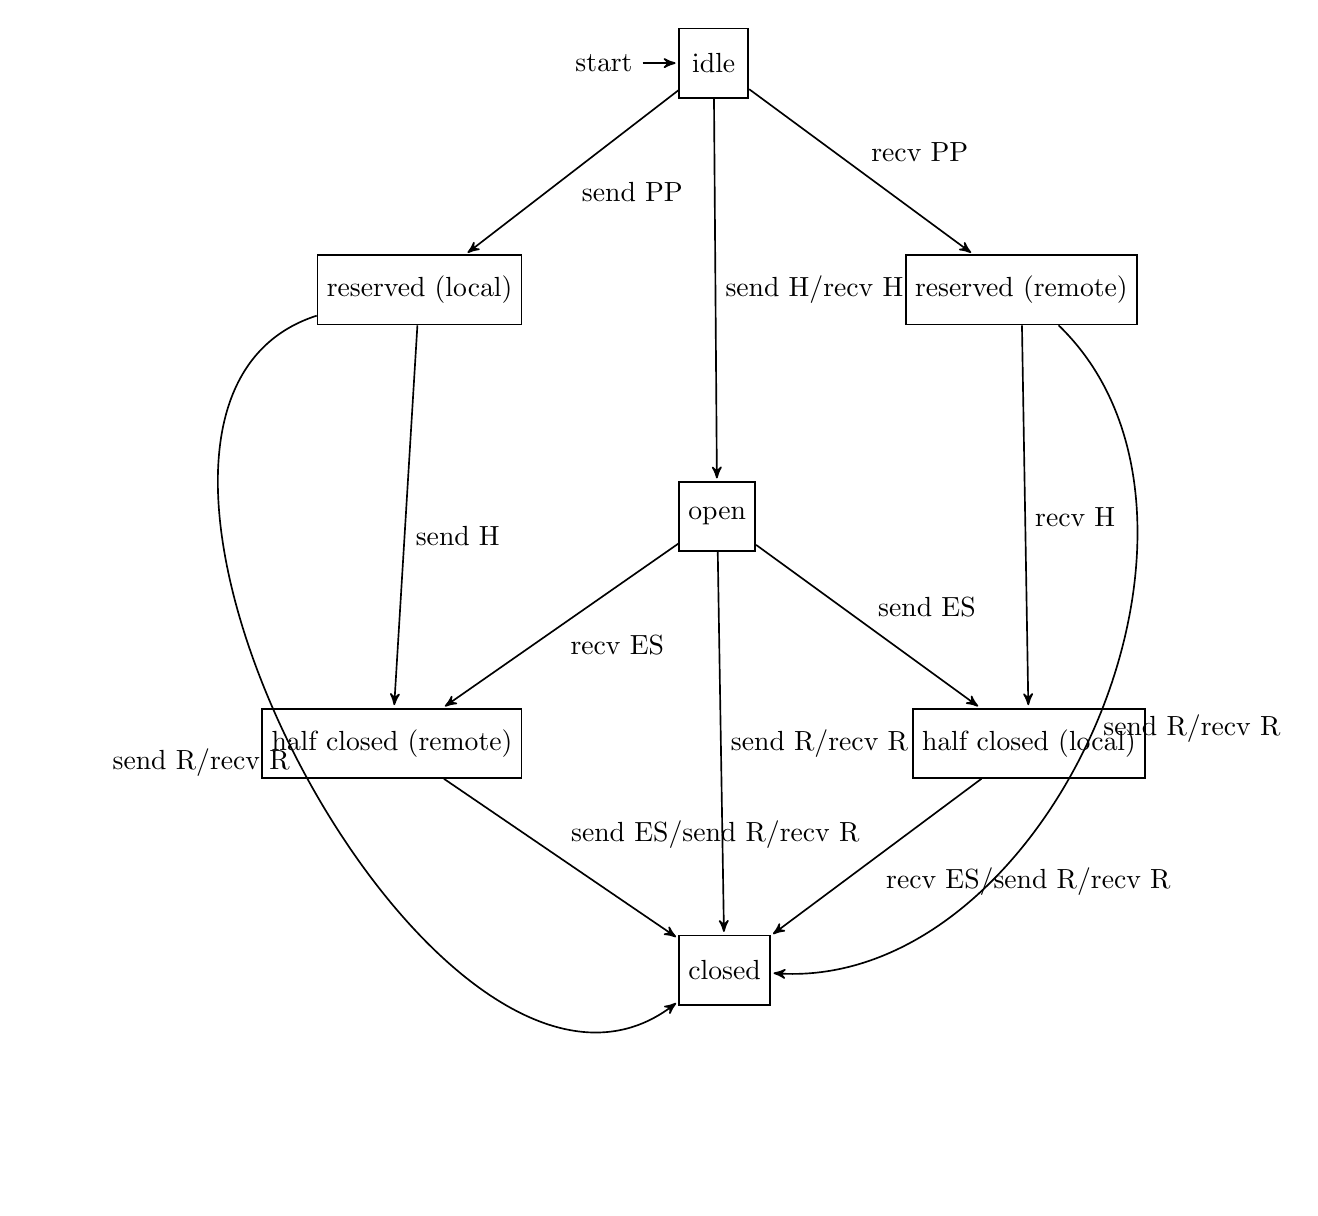
\begin{tikzpicture}[->,>=stealth',shorten >=1pt,auto,node distance=2.8cm,
                    semithick]
  \tikzstyle{every state}=[draw, rectangle]

 \node[initial,state](idle){idle};

 \node[state, below left =of idle](rsv_loc){reserved (local)};
 \node[state, below right= of idle](rsv_rem){reserved (remote)};
 \node[state, below right =of rsv_loc](open){open};

\node[state, below left=of open](hc_rem){half closed (remote)};
\node[state, below right=of open](hc_loc){half closed (local)};

\node[state, below right=of hc_rem](closed){closed};


 \path (idle) edge node {send PP} (rsv_loc)
         (idle) edge node {recv PP} (rsv_rem)
         (idle) edge node {send H/recv H} (open)
(rsv_loc) edge [bend right=100] node[left] {send R/recv R} (closed)
(rsv_rem) edge [bend left=70] node[right] {send R/recv R} (closed)
(rsv_loc) edge node {send H} (hc_rem)
(rsv_rem) edge node {recv H} (hc_loc)
(open) edge node {recv ES} (hc_rem)
(open) edge node {send R/recv R} (closed)
(open) edge node {send ES} (hc_loc)
(hc_rem) edge node {send ES/send R/recv R} (closed)
(hc_loc) edge node {recv ES/send R/recv R} (closed)
;

\end{tikzpicture}

http://http2.github.io/http2-spec/index.html\#StreamStates

\subsection{OpenSSL}


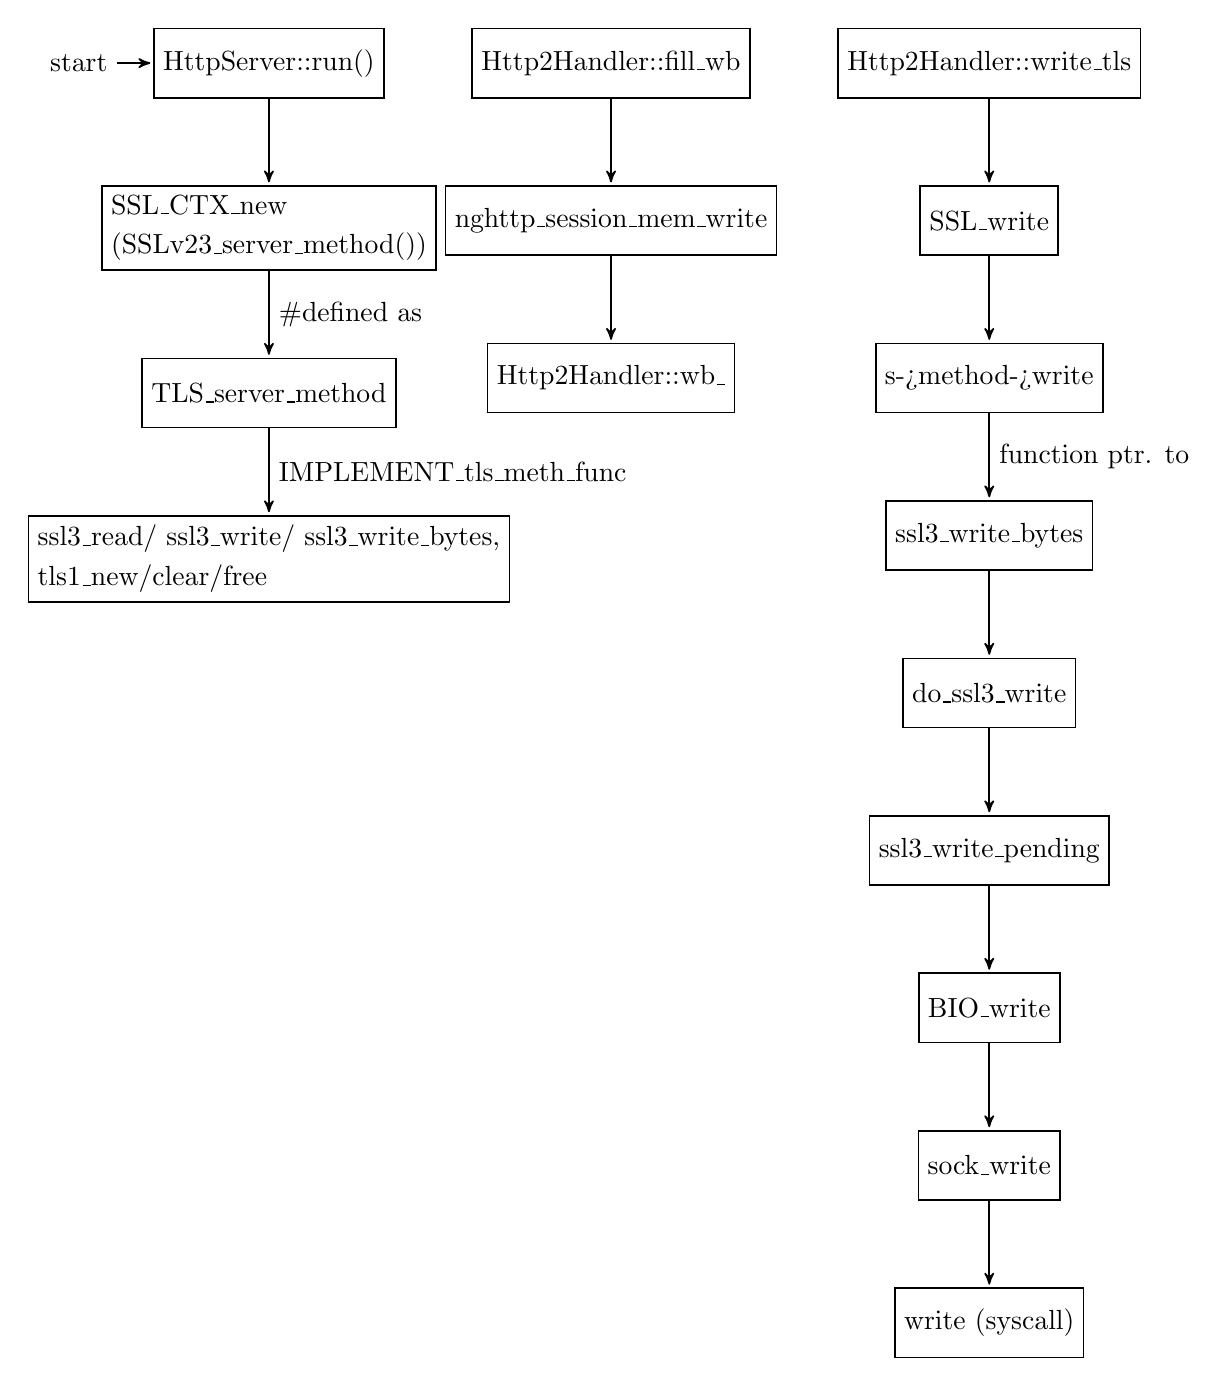
\begin{tikzpicture}[->,>=stealth',shorten >=1pt,auto,node distance=1.1cm,
                    semithick]
  \tikzstyle{every state}=[draw, rectangle,
   execute at begin node={\begin{varwidth}{21em}},
   execute at end node={\end{varwidth}}]

       \node[initial,state](s1){HttpServer::run()};
       \node[state,below=of s1](s2){SSL\_CTX\_new \\(SSLv23\_server\_method())};
       \node[state,below=of s2](s3){ TLS\_server\_method  };
       \node[state,below=of s3](s4){ ssl3\_read/ ssl3\_write/ ssl3\_write\_bytes, tls1\_new/clear/free };


 \node[state,right=of s1](s6){  Http2Handler::fill\_wb };
 \node[state,below=of s6](s7){  nghttp\_session\_mem\_write };
 \node[state,below=of s7](s8){  Http2Handler::wb\_ };



 \node[state,right=of s6](s9){  Http2Handler::write\_tls };
 \node[state,below=of s9](sa){  SSL\_write };
 \node[state,below=of sa](sb){  s->method->write };
 \node[state,below=of sb](sc){  ssl3\_write\_bytes };
 \node[state,below=of sc](sd){  do\_ssl3\_write };
 \node[state,below=of sd](se){  ssl3\_write\_pending };
 \node[state,below=of se](sf){  BIO\_write };
 \node[state,below=of sf](sg){  sock\_write };
 \node[state,below=of sg](sh){  write (syscall) };

\path (s1) edge (s2)
(s2) edge node {\#defined as} (s3)
(s3) edge node { IMPLEMENT\_ \\ tls\_meth\_func} (s4)

(s6) edge (s7)
(s7) edge (s8)

(s9) edge (sa)
(sa) edge (sb)
(sb) edge node {function ptr. to} (sc)
(sc) edge (sd)
(sd) edge (se)
(se) edge (sf)
(sf) edge (sg)
(sg) edge (sh)
;


\end{tikzpicture}


\section{Security Considerations}
The information passed from the HTTP server to the MPTCP scheduler creates a side channel bypassing TLS encryption. It needs to be considered whether the passed data or the observable scheduler decisions based on this data could help an adversary. Some information are only protected by HTTP/2 and would be exposed on HTTP/1.1 connections anyway, like the length of individual resources. Others, like the content type, might be not available to the attacker otherwise.

\section{Outlook / Future Work}



\section{Conclusion}



\renewcommand\refname{References}
\bibliography{thesis-h2-mptcp}{}
\bibliographystyle{plain}
\nocite{*}



\end{document}
